%
% CITI Research Report Template
%
% 07/2012: Paul Ferrand - Initial Template
% 02/2013: Frederic Le Mouel - Refactoring
% 

\documentclass[a4paper]{article}

%
  
\usepackage{pdflscape}
\usepackage{multirow}
\usepackage[utf8]{inputenc}% ou \usepackage[latin1]{inputenc}
\usepackage[T1]{fontenc}
\usepackage{lmodern}
\usepackage{graphicx}
\usepackage{listings}
\usepackage[bookmarks]{hyperref}
\usepackage{caption}
\usepackage{adjustbox}
\usepackage[section]{placeins}


\lstset{numbers=left, numberstyle=\small, numbersep=8pt, frame=single, framexleftmargin=15pt, columns=fullflexible,basicstyle=\ttfamily, breaklines=true,  tabsize=2}

\begin{document}

%
% Cover Page
%

\pagestyle{empty}
\begin{center}
\begin{figure}%
\centering
%
\includegraphics[width=0.5\columnwidth]{logo/citi-old-bw.eps}% old logo
%
\includegraphics[width=0.4\columnwidth]{logo/citi-new-bw.eps}% new logo 
%
\includegraphics[width=0.4\columnwidth]{logo/citi-new-title-bw.eps}% old logo - titled

\includegraphics[width=0.4\columnwidth]{logo/insa-noir.eps}
\end{figure}
%{\LARGE \textsc{Communication scientifique}} \\ % in French
{\LARGE \textsc{End of Study Project report}} \\ % in English
\vspace{0.5cm}
%{Centre d'Innovation en Télécommunications et Intégration de Services} \\ % in French
%{Center of Innovation in Telecommunications and Integration of Services} \\ % in English
{INSA Lyon - Telecommunications, Services \& Uses} \\
\vspace{2cm}
{\Large \textbf{Congolo: A Context-oriented language based on Golo language}} \\
\vspace{10pt}
{\large \textit{Baptiste Maingret}} \\
{\large \textit{Supervisor : Frédéric Le Mouël}} \\
\vspace{10pt}
{\large September 2014} \\
\vspace{20pt}
\begin{minipage}{0.8\columnwidth}
\sffamily
\small
Context-oriented programming (COP) ease the implementation of context-dependent behaviors. However they only allow for static definition of these variations with event-condition-action like decisions. We propose to separate the context-dependent variations and the system that will decide which variation to use based on the current context. For this purpose, we introduce two distinct context types: meta-values and concrete values, and the overall architecture is driven by events to help the separation of the two aspects cited above. We propose an implementation that uses the JVM dynamic language Golo and Java. To test our work we propose a web of things use case. From this we conclude that our proposition is adequate for this type of applications because of its ease of development, its light weight and the enhance decision-making system. In this paper, we present the Congolo language as well as the Java API supporting our contributions. We then give an overview of the implementation of a proof-of-concept for both. Finally, we discuss the use case and the results drawn from it.
\end{minipage}
\end{center}
\vfill
\begin{minipage}[b]{0.3\columnwidth}
\includegraphics[width=\columnwidth]{logo/sjtu_logo.jpg}%
\end{minipage}
\hfill
\begin{minipage}{0.3\columnwidth}
\small
\centering
\textbf{
%University of Lyon \\ % in English
INSA Lyon \\ % in English
Shanghai Jiao Tong University
}
\end{minipage}
\hfill
\begin{minipage}[b]{0.25\columnwidth}

\includegraphics[width=\columnwidth]{logo/insa-noir.eps}%
\end{minipage}

\newpage

%
% Title page
%

\title{Research Report}

\author{Baptiste Maingret\\[10pt]
INSA-Lyon, F-69621, Villeurbanne, France\\
\texttt{baptiste.maingret@insa-lyon.fr}}

\date{\today}
\newcommand{\Keywords}[1]{\par\noindent 
{\small{\em Keywords\/}: Context-Oriented Programming, Golo, Java, System reasoning, Dynamic Language}}
\maketitle

\begin{abstract} 
Context-oriented programming (COP) ease the implementation of context-dependent behaviors. However they only allow for static definition of these variations with event-condition-action like decisions. We propose to separate the context-dependent variations and the system that will decide which variation to use based on the current context. For this purpose, we introduce two distinct context types: meta-values and concrete values, and the overall architecture is driven by events to help the separation of the two aspects cited above. We propose an implementation that uses the JVM dynamic language Golo and Java. To test our work we propose a web of things use case. From this we conclude that our proposition is adequate for this type of applications because of its ease of development, its light weight and the enhance decision-making system. In this paper, we present the Congolo language as well as the Java API supporting our contributions. We then give an overview of the implementation of a proof-of-concept for both. Finally, we discuss the use case and the results drawn from it.
\Keywords{Context-Oriented Programming, Golo, Java, System reasoning, Dynamic Language, Internet of things, Web of things}
\end{abstract}

\newpage

%
% Report Body
%

\section{Introduction}

Internet of Things (IoT) takes a lot of attention nowadays because of its implication in our daily lives, its market opportunities and also because of its unique technological requirements. Protocols have emerged to make the IoT a reality and today's trend is to standardize them to allow its further development and ease of interconnection with existing infrastructures. Thus the Web of Things is also taking interest because of the ease of development, its well-known standard and the numerous existing web-based systems. On the other side, software development for IoT has not seen many improvements nor recent evolution to cope with the new specifications of IoT such as mobility, changing environment, dynamism...

In parallel context-oriented programming (COP) has drawn research interest in the past years and as a result several new COP languages have emerged. Most of these approaches allow for multiple context definitions and their activation. They also allow the developer to specify context-dependent behaviors. Because of the dynamism of the IoT, COP could be a good option for the development applications built upon it.

Many languages have seen their COP counterparts born. Several approaches were based on Java and the JVM. Because of its high development in embedded system, the JVM seems to be a good candidate for the development of IoT applications. In addition, dynamic languages for the JVM have been created such as Groovy or Golo \cite{ponge_golo_2013}, a lightweight dynamic JVM language built around the newly introduced invokedynamic \cite{jponge_invokedynamic_2013} instruction.  In \cite{appeltauer_layered_2010} the authors explores the use of the new INVOKEDYNAMIC (ID) instruction introduced in Java 7 which allows for dynamic method dispatch to implement the layer method dispatch in JCOP \cite{appeltauer_declarative_2013}. The performances shown are encouraging especially since at the time of writing the implementation of ID in the JVM was not yet over. Thus the Golo language, based on ID from day one, appeared to be a good applicant for a COP language.

The decision-making systems backing up these COP languages is usually simple and may have difficulties to cop with the requirements of IoT. Whereas it is to decide what context should be activated or what actions should be done based on the current context, current systems only allow for one implementation and does not provide any sort of abstraction. Systems are often simple event-condition-action (ECA) process which do not leverage the full potential of the IoT. More advanced systems such as neural networks, genetic algorithms or Petri net could be used.

In this paper we propose a new COP language named Congolo, extending the Golo language. In addition we propose a Java API that will provide an abstraction of the reasoning mechanisms, whether it is a simple event-condition-action (ECA), an automate, a neural network or yet another approach. To test our solution and put it into action, we will propose a use-case based on a WoT application.

In section \ref{section:problemstatement} we will first state the problem at hands before we see the different approaches taken by existing COP languages to explain the choices made in Congolo in \ref{section:stateoftheart}. In \ref{section:contribution} we will present Congolo and the abstraction mechanism for decision-making and reasoning systems. In \ref{section:implementation} we will describe the implementation and discuss the choices made. Based on this implementation, we will discuss a use-case and draw  some results in \ref{section:results}. Finally we will end up by a  discussion about this work in \ref{section:discussion} and conclude in \ref{section:conclusion}.

\section{Problem statement}
\label{section:problemstatement}
The progress and development made in embedded devices especially with the advent of the internet of things, faced developers with more complexity because of the diversity of the environment and context were  these devices evolve.

One solution developed to face this problem is COP. COP languages are designed to allow programmers to efficiently and easily define multiple variations and behaviors for a defined component based on some context is defined elsewhere. However we found that current works usually focus on the context part, which is a good thing, but lack the support for reasoning systems backing up the context processing and the corresponding context-dependent behaviors. They commonly used system is an ECA like system which doesn't allow for advanced reasoning.

For instance, take a simple light automation systems based on presence sensors. In an ECA manner, one could simply activate a context whenever someone is detected and that it is dark outside. But we could also use a learning algorithm backed up by a neural network so that the system would learn by itself of when and when not it should turn on the light. It could thus be easy to take more information into account, such as whether the television is turned on, which light to turn on, or learn from false positive (when the user would turn off the light after the system would have turned them on). In some of the current work, it could be done somehow by reasoning about the context information before each call to a contextual functions and thus finding the right context to activate. However we find this approach to be too verbose and maybe too much of an overhead for the programmer.

What we would like is to be able to declare a decision-making system from the beginning that would be used for each call to a contextual function. This would release the developer of explicitly using it and would better separate the two aspects of COP: layers and contexts. Indeed, on one side we would define several context-dependent functions that could be called depending on the context. On the other side the context would be defined by a different system that once the needed information retrieved will decide which context to activate and thus which function to call.

\section{State of the Art}
\label{section:stateoftheart}
\paragraph{Context-Oriented Programming}
There are already many COP languages based on a variety of languages. Most of them implements the context with the use of layers which act as a context and context-dependent behaviors definition but some others also explicitly separate the two. In order to compare these languages we can thus focus at first on the way the context are defined, then how they are activated and finally how they are used throughout the code. A summary table \ref{table:coplanguages}, inspired by \cite{appeltauer_comparison_2009}, is proposed.

In many languages, context is integrated directly in the business code by the mean of layers. It is the case in JCop \cite{appeltauer_declarative_2012}, as in listing \ref{listing:jcoplayer}, ContextJ \cite{appeltauer_dedicated_2008} \cite{appeltauer_improving_2009}, ContextErlang \cite{ghezzi_context_2010}, ContextLua \cite{wasty_contextlua:_2010} or EventCJ \cite{kamina_eventcj:_2011}. In ECaesarJ \cite{nunez_declarative_2009}, NextEJ \cite{kamina_towards_2009} or Javanese \cite{kamina_unified_2013} the contexts are declared separately as in listings \ref{listing:ecaesarjcontext}, \ref{listing:javanesecontext} and \ref{listing:nextejcontext}. In EventJava \cite{jayaram_context-oriented_2009}, context is considered to be an event with specific data, listing \ref{listing:eventjavacontext} and is defined alongside the event consumer. Thus when the event arrives, the context is embedded into it.

\begin{lstlisting}[float, language=Java, caption=JCop layer example, label={listing:jcoplayer}]
public class Hero {
  public Point getPosition() {...} //plain meth.
  public void move(Direction dir) {...} //base meth. for layered method Hero.move
  private Position getPos() {...} //base meth. for layered method Hero.getPos
  
  layer ConfusedHeroLayer { //layer extension declaration
    private Position getPos() {...} //partial meth. for layered method Hero.getPos
  }

  public layer ConfusedHeroLayer { //(top-level) layer declaration
    public void Hero.move(Direction dir) { //partial meth. for layerd meth. Hero.move
      proceed(dir); //a proceed expression
    }
    private Direction getNewDir(Direction original) {...} //layer local method
  }
}
\end{lstlisting}

\begin{lstlisting}[float, language=Java, caption=ECaesarJ context declaration, label={listing:ecaesarjcontext}]
cclass ScheduledNightTime extends Context {
  TimeService sunset, sunrise;
  event in() = sunset.time();
  event out() = execution(* *.openBinds(..));
  // or
  //  event out() = sensor.intensityChanged(int i) && if (isActive() && i > threshold);
}
\end{lstlisting}

\begin{lstlisting}[float, language=Java, caption=Javanese context declaration, label={listing:javanesecontext}]
// Contexts declaration
context GPSon
  active(int s) :after call(void Nav.onStatusChanged(*)) && args(s)
      && if(GPS.AVAILABLE==s)
  until(int s) :after call(void Nav.onStatusChanged(*)) && args(s)
      && if(GPS.AVAILABLE!=s);
      
context RouteSearching
  // context active during the execution of the specified method
  cflow(call(void Nav.calcRoute()));
\end{lstlisting}

\begin{lstlisting}[float, language=Java, caption=NextEJ context declaration, label={listing:nextejcontext}]
context Building {
  role Guest {
    void escape() { .. }
  }
  role Security {
    void notify() {
      Guest.escape();
    }
  }
}
\end{lstlisting}

\begin{lstlisting}[float, language=Java, caption=EventJava context declaration, label={listing:eventjavacontext}]
public class Context implements Comparable<Context>, Serializable {
  public long time;
  ... /* more fields */
  public Context() { time = System.currentTimeMillis(); }
  public Context(long time) { this.time = time; }
  public int compare(Context other) {
    if(timestamp == other.timestamp) return 0;
    ...
  }
  ...
}
\end{lstlisting}

The activation of the context, or layers depending on the language, often use the keyword \lstinline|with| \cite{haupt_contextj:_2011} \cite{appeltauer_declarative_2013} \cite{kamina_towards_2009} \cite{wasty_contextlua:_2010} as shown in the listing \ref{listing:jcopwith}. Instead \cite{ghezzi_context_2010}, \cite{nunez_declarative_2009} or \cite{kamina_eventcj:_2011} use a different approach where contexts are activated independently of the running program by the mean of events. In \cite{nunez_declarative_2009}, the activation is done by the use of specific events declared in the context object which can be triggered by others events, by method invocation or by composite expression as in listing \ref{listing:ecaesarjcontext}. In \cite{kamina_eventcj:_2011}, they declare transition rules based on events that will activate or deactivate contexts, as in listing \ref{listing:eventcjevent}. In \cite{kamina_unified_2013}, where the distinction is made between context and layers, the context state is changed by specific actions and thus can be activate in the program, whereas layers are activated according to the state of one or multiple contexts and thus are activated implicitly, as in listing \ref{listing:javanesecontext}. Finally in \cite{jayaram_context-oriented_2009} where the context is defined by specific values of information when the event is triggered, the activation of the context is global but its particular definition, i.e. the values of the information that it holds, are defined by events.

 
\begin{lstlisting}[float, language=Java, caption=JCop layer activation, label={listing:jcopwith}]
public void moveHeroLeft() {
	with (new ConfusedHeroLayer(), new RainLayer()) {
    getHero().move(Direction.LEFT); }
}
\end{lstlisting}

\begin{lstlisting}[float, language=Java, caption=EventCJ layer activation, label={listing:eventcjevent}]
direction SwitchPositioningDevice {
  declare event GPSEvent(Navigation n, int s)
    :after call(void Navigation.onStatusChanged(s))
      &&target(n)&&args(s)
      &&if(s==LocationProvider.AVAILABLE)
    :sendTo(n);
  declare event WifiEvent(Navigation n, int s)
    :after call(void Navigation.onStatusChanged(s))
      &&target(n)&&args(s)
      &&if(s==LocationProvider.OUT_OF_SERVICE)
    :sendTo(n);
  declare event Boarding()
    :after call(void *.cabinModeEntered());
  declare event Arriving()
    :after call(void *.cabinModeExit());
  
  transition GPSEvent:
    WifiNavi switchTo GPSNavi | not OnBoard activate GPSNavi;
  transition WifiEvent:
    GPSNavi switchTo WifiNavi | not OnBoard activate WifiNavi;
  transition Boarding:
    * switchTo OnBoard;
  transition Arriving:
    OnBoard switchTo .;
}
\end{lstlisting}

\begin{lstlisting}[float, language=Java, caption=Javanese context declaration, label={listing:javaneselayer}]
// Layers declaration
activate Outdoors when GPSon && StrongGPS;
activate Indoors when !GPSon || !StrongGPS;
\end{lstlisting}

Finally, we need to consider how the rest of the program takes into account the different contexts to adapt and modify the program. Two strategies are often found when the language use a layer paradigm: layer-in-class and class-in-layer implementation, but only the first one is usually implemented. In the first one, the layers and corresponding behaviors are implemented inside the class such as in \cite{appeltauer_improving_2009} \cite{appeltauer_declarative_2013} \cite{wasty_contextlua:_2010} (listing \ref{listing:jcoplayer}) or as in \cite{kamina_eventcj:_2011} \cite{kamina_unified_2013} (listing \ref{listing:eventcjlayeruse}). \cite{kamina_towards_2009} follows the same approach but differs by the fact that they use roles defined in the context classes to implement the different behaviours. \cite{ghezzi_context_2010} states that both methods have their advantages and thus offers the possibility of using the both of them. ECaesarJ offers two distinct ways of using the current context. First, it is possible to bind specific events to the events triggered by the context changes as in listing \ref{listing:ecaesarjcontextuse} or to directly query the context state with the help of the method \lstinline|isActive()| of the context. In \cite{jayaram_context-oriented_2009}, as the context is represented by variables bound to an events, the context-dependent behaviors are implemented using this data such as in listing \ref{listing:eventjavacontextuse}.

\begin{lstlisting}[float, language=Java, caption=ECaesarJ context use, label={listing:ecaesarjcontextuse}]
cclass LightAutomation {
  ILight light;
  Context context;

  event mustTurnOn() = context.in();
  event mustTurnOff() = context.out();

  mustTurnOn() => { light.switchOn(); }
  mustTurnOff() => { light.switchOff(); }
}
\end{lstlisting}

\begin{lstlisting}[float, language=Java, caption=EventCJ context-dependent behaviour, label={listing:eventcjlayeruse}]
class Navigation extends MapActivity implements Runnable, LocationListener {
  MapView mapView;
  MyLocationOverlay overlay;
    
  void onStatusChanged(...) {...}
  void run() {}
  void onCreate(Bundle status) {
    overlay.runOnFirstFix(this);
  }
  
  layer GPSNavi {
    activate { overlay.onProviderEnabled("gps"); }
    deactivate { overlay.onProviderDisabled("gps"); }
    after void run() {
      Location loc = overlay.getMyLocation();
      mapView.getController().animateTo(loc);
  }
}
\end{lstlisting}

\begin{lstlisting}[float, language=Java, caption=EventJava context-dependent behaviour, label={listing:eventjavacontextuse}]
public class Context implements Comparable<Context> , Serializable {
	public long time;
	public float latitude; //in decimal degree format
	public float longitude; //in decimal degree format
	... //more fields and methods
}

class AnimalMonitor1 {
	float currLatitude;
	float currLongitude;
	2DPoint loc = new 2DPoint(currLatitude, currLongitude);
	event animalLocation[10](long animalID, String family) when
		( for i in 0..8 animalLocation[i].animalID == animalLocation[i+1].animalID &&
		for i in 0..9 euclideanDistance(loc, new 2DPoint(animalLocation[i].latitude, animalLocation[i].longitude)) > 0.5 &&
		animalLocation[9].time - animalLocation[0].time <= 60*60*1000) {
			triggerAlert("Animal " + animalID + " out of safety zone ");
		}
}
\end{lstlisting}

One can encounter different type of implementation for COP languages. The easiest one might be to develop an API such as \cite{appeltauer_dedicated_2008}. One can also extends existing languages with new keywords such as in \cite{clarke_semantics_2009}, ContextJ \cite{haupt_contextj:_2011}, JCOP \cite{appeltauer_declarative_2013}, NextEJ \cite{kamina_towards_2009} or \cite{ghezzi_context_2010}. Finally some papers propose a new COP language as  EventCJ \cite{kamina_eventcj:_2011} or \cite{kamina_unified_2013}.

\begin{landscape}
  \begin{table}
  \begin{adjustbox}{center}
  \begin{tabular}{l p{3cm} c c c c c c c c c c}
  \hline
  \multicolumn{2}{l}{Languages} & ContextJ & JCop & EventCJ & NextEJ & ContextLua & ContextErlang & EventJava & Javanese & ECaesarJ \\

  \hline
  \multirow{2}{*}{Context declaration}
    & Layer &   X & X & - & - & X & X & - & - & - \\
    & Class &   - & - & X & X & - & - & X & X & X \\
    
  \hline
  \multirow{2}{*}{Context type}
    & State &   X & X & X & X & X & X & - & X & X \\
    & Data  &   - & - & - & - & - & - & X & - & - \\    

  \hline  
  \multirow{2}{*}{Layer declaration}
    & Layer-in-class &   X & X & X & X & X & X & X & X & X \\
    & Class-in-layer &   - & - & - & - & - & X & - & - & - \\

  \hline
  \multirow{2}{*}{Layer implementation}
    & Class &       - & - & - & - & - & - & - & X & X \\
    & Layer type &  X & X & X & X & X & - & - & X & - \\    

  \hline  
  \multirow{3}{*}{Scope}
    & Instance &        - & - & X & - & X & - & X & X & X \\
    & Thread &          X & X & - & - & - & - & X & X & - \\
    & Dynamic extent &    &   &   &   &   &   &   &   &   \\
    & Global &          - & - & - & - & - & X & X & X & - \\

  \hline
  \multicolumn{2}{l}{Events/messages supported}
    & - & - & X & - & - & - & X & X & X \\

  \hline
  \multirow{2}{*}{Active context tracking}
    & Push to layer stack &             X & X & X & - & - & X & X & X & - \\
    & Directly change method lookup &   - & - & - & - & - & - & X & - & - \\

  \hline    
  \multirow{3}{*}{Implementation}
    & Language extension &   X & X & - & - & X & X & X & X & - \\
    & New language &         - & - & X & - & - & - & - & X & - \\

  \end{tabular}
  \end{adjustbox}
  \caption{COP languages comparison}
  \label{table:coplanguages}

  \end{table}
\end{landscape}


\paragraph{Decision-making systems}
Decision making is the process of outputting a final choice based on inputs, that could result in an action. There are several approaches that we can at first separate into two groups based: fixed-design and machine learning.

Basic systems such as event-condition-action (ECA), state transition systems or Petri net allow basic decision making. They do not require any training and only a basic initialization. In most of the COP languages cited above, ECA is used for the layers activation.

More advanced systems of machine learning can be used for decision making. These include artificial Bayesian networks, cluster analysis techniques, particle swarm, simulated annealing, support vector machine, decision-tree learning, association rule learning, similarity and metric learning, sparse dictionary learning, artificial neural networks (ANN), genetic algorithms... They usually are classified in three categories, each of them allowed to belong to more than one, based on the type of learning that can be used to initialize the system: supervised, unsupervised and reinforcement as summarized in table \ref{table:machinelearning}.

\begin{table}[bt]
\begin{tabular}{l c c c }
\hline
\multirow{2}{*}{Languages} & \multicolumn{3}{c}{Learning method} \\

 & Supervised	 & Unsupervised	& Reinforcement \\

\hline
Bayesian Networks	             & X & - & - \\

\hline
Clustering	                     & - & X & - \\

\hline
Genetic Algorithms             & - & - & X \\

\hline
Artificial Neural Networks     & X & X & X \\

\hline
Particle Swarm Optimization    & X & - &	- \\

\hline
Simulated Annealing            & X & - &	- \\

\hline
Support Vector Machines        & X & - & - \\

\hline
Decision Tree Learning         & X & - &	- \\

\hline
Association Rule Learning      & - &	X &	- \\

\hline
Similarity and Metric Learning & X &	- &	- \\

\hline
Sparse Dictionary Learning     & X & X &	- \\
\end{tabular}

  \caption{Machine learning methods}
  \label{table:machinelearning}
\end{table} 

From an implementation point of view, there are languages which are often used for artificial intelligence development and thus tend to be used to design decision making systems. Such languages include Lisp and its derivatives, and Prolog. However none of them include context-oriented functionality and there does not seem any extension for COP to exist even if aspect oriented have been researched using Prolog \cite{lohmann_aspect-oriented_2008}. In addition to these dedicated languages, we can find AI frameworks such as the Encog Machine Learning Framework (EMLF) which implements a wide variety of AI process but they still do not allow for an abstraction regarding the type of algorithm to be used.

So on overall, we can see that there are many decision making systems that could be used and benefit the IoT but that there are no integration with COP languages form which the IoT could also benefit, hence our proposition.

\goodbreak
  \section{Contribution}

\label{section:contribution}

In this paper we propose a new COP language, namely Congolo, based on the Golo language \cite{ponge_golo_2013}. We offer COP functionalities based on the study of previous papers and existing solutions. We also introduce a new way of abstracting the decision making process with the help of a Java API integrated into the language.
\subsection{Context management}
\label{subsection:contextmanagement}

As seen in section \ref{section:stateoftheart}, most papers handle context as a simple state system where contexts are two-state variables that can either be activated or deactivated. In our case, we decided to allow a more flexible way of handling the context by introducing two levels of context values: meta values and concrete values. The meta values are used into the business code to declare the different layers (to be understood as defined by other papers). On the other hand, concrete values are used inside the decision-maker that will output the meta values based upon these and thus decide which layers to activate, as in Figure \ref{figure:concretemetavalues}. Hence the context is not directly activated but concrete values are used to determine it with the help of a decision-maker. The current state of the context is thus represented by the current concrete values whose scope is for now only on the Golo module level. The declaration of a context in Congolo is done using the keyword \lstinline|context| as shown in listing \ref{listing:congolocontext}. The following expression must be a tuple composed of class instances implementing the Context interface defined in the Congolo API.

\begin{lstlisting}[float, language=Java, caption=Congolo context example, label={listing:congolocontext}]
contexts  =  [ConfusedHero(), Weather()]
\end{lstlisting}


\begin{center}
\begin{figure}
\centering
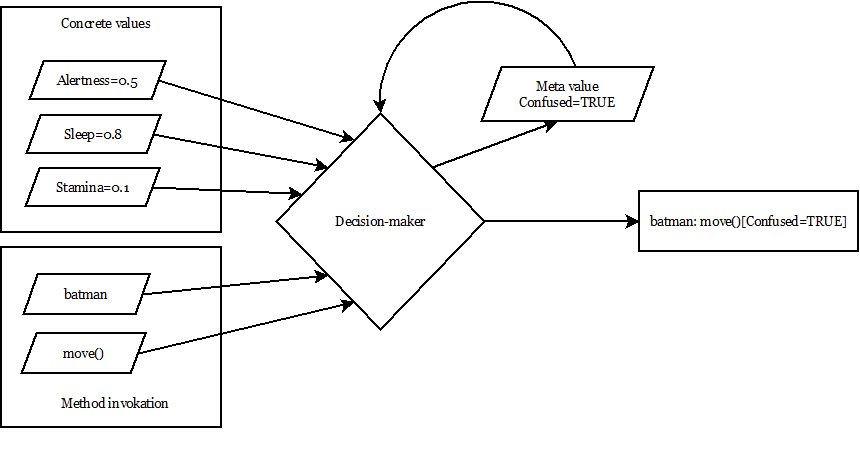
\includegraphics[width=0.9\columnwidth]{images/concrete-meta-values.png}
\caption{Concrete and meta values in context representation}
\label{figure:concretemetavalues}
\end{figure}
\end{center}

\subsection{Layers}
\label{subsection:layers}
Layers are usually defined as alternative methods to base methods (that are context independent) that will eventually be triggered depending on the context. The declaration is done with the help of a keyword such as \lstinline|layer|, allowing to define multiple methods belonging to one layer. In our case, we propose an alternate method definition to indicate layers by using the arobase symbol and appending them to the method's parameter list: \lstinline!function myFunc = |arg1|@(contextA=METAVALUE1)! as in listing \ref{listing:congololayers}. This choice was made because of the compatibility of this definition with the different function definition allowed by Golo and because we think it looks like it really belongs to the language rather than having been added in an ad-hoc manner.

In other languages, it is usually possible to call the base method from the layered one. We propose this in a similar manner by using the keyword \lstinline|proceed()| that will refer to the base method from the layered one. In addition we propose syntactic support for two basic cases where the developer wish to call the base method before or after the layer as shown in listing \ref{listing:congololayers}.

When multiple layers are activated at the same time, the usual proposed way is to simply take them in a LIFO manner as if they were stacked. However in our case the method to be called is chosen by the decision-maker. Thus in the case were multiple contexts, i.e. multiple meta values, are activated at the same time, again the system will make the decision to chose which methods are to be called.

\begin{lstlisting}[float, language=Java, caption=Congolo layers example, label={listing:congololayers}]
function Hero = || {
  return DynamicObject():
    contexts([ConfusedHero, Weather]):
    define("getPosition", |this| -> ...): # plain method
    define("move", |this, dir| -> ...):   # base method
    define("getPos"; |this| -> ...):    # base method
    #layer declaration, invoked before base method
    define("getPos", |this, direction|@(ConfusedHero=TRUE)+ -> ...):
    # layer method, invoked after base method
    define("move", |this, dir|+@(ConfusedHero=TRUE) -> ...):
    # layer method, with a call to the base method from within the layer
    define("move", |this, dir|@(ConfusedHero=TRUE) = {
      ...
      proceed(dir)
      ...
    }
}
\end{lstlisting}

\subsection{Decision maker}
\label{subsection:decisionmaker}

One singular aspect of our proposition regarding previous ones is the way layers are activated. In previous papers, it was usually done in an ECA manner: when a specific context is activated and that a layered method is invoked, the corresponding layer is used. In that case, the decision is made at the programming step. It is of course possible to dynamically change the context at runtime but its binding to the layers is still static. In our case, we propose to delegate this decision to an external system, the decision-maker (DM), which could be static just as in others papers but could also be based on more advanced algorithms and techniques from machine learning such as neural networks or genetic algorithms.  In this case, the system could actively learn during the runtime of the application. We offer two ways of defining which DM is to be used to resolve the method to invoke. First it is possible to have a specific DM per object, and declaring it by defining a \lstinline|desisionmaker| attributes in a dynamic object using a reference to an instance of a class implementing the Java interface \lstinline|fr.insa.lyon.congolo.api.DecisionMaker| as in listing \ref{listing:congolodecisionmaker1}.

\begin{lstlisting}[float, language=Java, caption=Congolo decision maker definition, label={listing:congolodecisionmaker1}]
function Hero = |decisionMaker| {
  return DynamicObject():
  decisionmaker(decisionMaker)
}

let misterPresident = my.app.myDecisionMaker()
let batman = Hero(misterPresident)
\end{lstlisting}

\begin{lstlisting}[float, language=Java, caption=Congolo example, label={listing:congolohero}]

let misterPresident = my.app.myDecisionMaker()
misterPresident: global(true)

let batman = Hero() # Context-dependent object
batman: move()        # Call to a layered method that will be handle by one of the global decision-maker

\end{lstlisting}

In order to further separate the decision-making process from the rest of the application, we propose that the decision-makers use events as primary inputs and outputs. This events can either contains data, such as data from the concrete values, object and method for method invocation, or context information (meta values). In addition, the output can either be a method invocation, corresponding to the decision made by the system, or an event that could be further used as an input for the system.

\section{Implementation: from Golo to Congolo}
\label{section:implementation}
In this section, we will detail the implementation of the proof-of-concept (PoC) we developed. It comes with a limited set of functionality and does not follow exactly the requirements of the contributions in terms of syntax or integration but the main aspect which is the separation between the decision-making system and the rest of the code is working and it is still sufficient to develop a simple use case and start to draw some results. 

\subsection{Context support in the language}
To provide the support for layered methods, we first modified the grammar of the language to introduce the corresponding elements as shown in \ref{listing:implgrammar}, and then modified the AST representation \lstinline|fr.insalyon.citi.golo.compiler.parser.ASTFunction| to support the added context information. The grammar is defined using JJtree, a preprocessor for JavaCC.

\begin{lstlisting}[float, language=Java, caption=Grammar modification - Golo.jjt, label={listing:implgrammar}]
void Function():
{
  List<String> arguments = null;
  Token varargsToken = null;
  boolean compactForm = false;
  List<String> contexts = null;
  boolean contextual = true;
}
{
  ("|" arguments=Arguments() (varargsToken="...")? "|")?
  ("@(" contexts=Contexts() ")")?
  ...
}
\end{lstlisting}

To support multiple function definition in a same module, we used a renaming convention so that a function with a context information would be renamed as \lstinline|originalFunctionName__$context$__context|.  Golo use an intermediate representation (IR) to ease the compiling process, see Figure \ref{figure:congoloparsing} and we implemented this part at the translation from the ASTtree to this IR representation in the \lstinline|fr.insalyon.citi.golo.compiler.ParseTreeToGoloIrVisitor| class.

\begin{lstlisting}[float, language=Java, caption=IR modification - ParseTreeToGoloIrVisitor.java, label={listing:implastfunction}]
public Object visit(ASTFunctionDeclaration node, Object data) {
  ...
  if ((child instanceof ASTFunction) && (((ASTFunction) child).isContextual())) {
    nodeName = node.getName() + "__$context$__" + ((ASTFunction) child).getContexts().get(0);
  }
  ...
}
\end{lstlisting}

\begin{center}
\begin{figure}
\centering
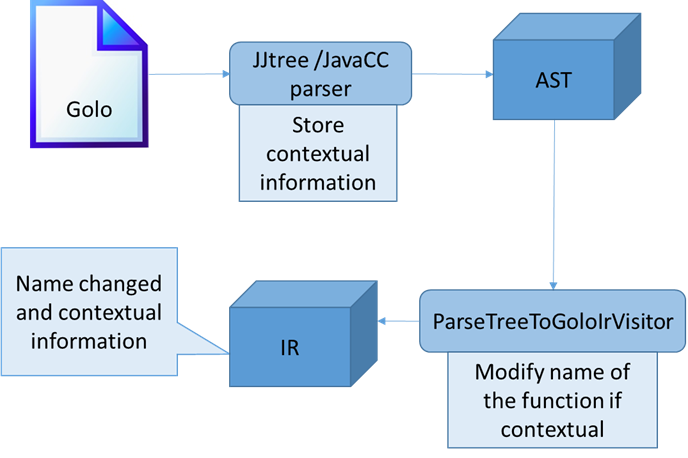
\includegraphics[width=0.9\columnwidth]{images/congolo_parse.png}
\caption{Congolo parsing process}
\label{figure:congoloparsing}
\end{figure}
\end{center}

\subsection{From function call to the decision system}

In order to abstract and decouple the DM from the rest of the code, we opted for an event-oriented system, as in Figure \ref{figure:congoloinvoke}. But to be able to use we first needed to add the support for contextual function invocation to Golo so that we could trick it as we wanted afterwards. We implemented this in the compilation process of Golo, whereas the decision-maker is designed as a Java API.

\subsubsection{Custom boostrap method}
First to be able to call the contextual function by their original given name, we changed the function invocation of contextual functions. Golo is based on the invokedynamic opcode to bind at the runtime the callsite to the correct target, as defined by the language. For this process it provides several utility classes in the \lstinline|fr.insalyon.citi.golo.runtime| package that acts accordingly to their name; FunctionCallSupport, MethodInvocationSupport, etc. We thus extended this package with the new class \lstinline|ContextualFunctionCallSupport|. The Golo compiler replace function calls, in the most generic terms of that, by invokedynamic instruction that are bound to specific bootstrap utility class according to their type (method, function, closure). In order to be able to use our newly designed bootstrap class we thus need to identify which of the function calls correspond to contextual function calls. We make this identification in the \lstinline|LocalReferenceAssignmentAndVerificationVisitor| class. We already know which functions are contextual so we build a list containing those so that we can latter check whether the name of the invoked function matches the name of a contextual function and marking it as such. Then in the bytecode generation process we simply use our custom bootstrap class for those function calls.

The contextual bootstrap method then wrap everything into a message that will be send to the decision maker. Since the call needs to be synchronized (the bootstrap method should return a method handle that will later be used at the original callsite, we then block the current thread waiting for the answer from the DM. The bootstrap class actually reacts on a specific type of message that triggers a function that will unlock the thread and finally configure the method handle according to the decision made by the DM. Once the bootstrap method is made the call site is bound to the correct target as for the DM.

\subsubsection{Event messaging}
The messaging system used is a simple hierarchical-namespace messaging system developped especially for Golo \cite{flemouel_gololang-messaging_2013}. These events are used to make the link between the function call and the DM. The implementation is multi-threaded and the hierarchical design allows for interesting behaviors for a COP languages. It will be indeed easy to reach multiple decision-makers, or implement various scope for the contexts.

The framework either used a callback mechanism where you can register a specific handle to be invoked upon the reception of the message, or an interface one where you register an instance of a class implementing the \lstinline|gololang.concurrent.messaging.MessagingFunction|.

\subsubsection{The decision maker}
The decision-making part is designed as a Java API that defines a common \lstinline|DecisionMaker| interface. We also provided a \lstinline|DefaultDecisionMaker| class that implements some basic needed functionality allowing to quickly test our solution. The interface require the implementation functions such as \lstinline|train| or \lstinline|init| but which are not used in our implementation because of its simplicity. They would be used in more advance systems such as a neural network. 

\begin{center}
\begin{figure}
\centering
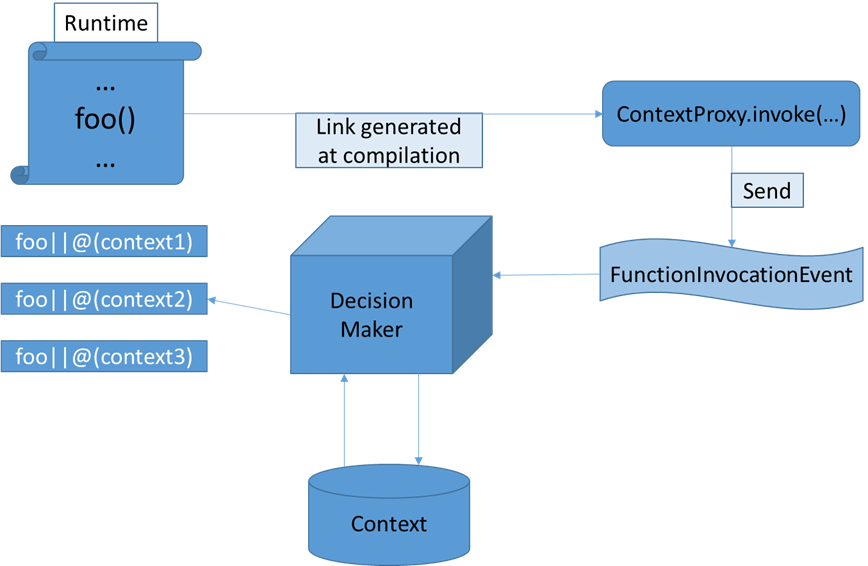
\includegraphics[width=0.9\columnwidth]{images/contextual_invocation.png}
\caption{Congolo invocation process}
\label{figure:congoloinvoke}
\end{figure}
\end{center}

\subsection{Context management}
To be done

\section{Use case and results}
\label{section:results}
The evaluation of programming languages can be difficult. Benchmarks are a common way of doing this, but there usually are pitfalls because of the numerous options of compilation or runtime, the type of hardware, the versions of software and so on. In COP languages, a common benchmark is to compare calls to layered functions versus calls to standard functions and see the ovehead such as described in \cite{appeltauer_comparison_2009} where multiple languages were tested to create a benchmark. To do so they compare 10 methods layered to plain implementation. An alternative is to compare the verbosity and/or the ease of programming between languages. For instance, \cite{appeltauer_declarative_2013} compare JCOP to the previous ContextJ and notice a significant reduction of code due to layer inheritance mechanism and context classes to better compose layers. We will try to evaluate both aspects by first reviewing the results of small microbenchmarks achieved using the JMH framework. Then we will describe a small use case and compare Congolo to Golo and Java.

\subsection{Performance evaluation: micro-benchmarks}


\subsection{Language comparison: Congolo versus Golo versus Java}

To test our PoC, we decided to implement a small farmhouse simulation. The farmhouse is composed by multiple greenhouses that embedded a temperature sensor. The is also an actuator that allow to change the heater temperature.

We designed a simple system where the temperature sensors would update the context information about the temperature of the greenhouse. Then each period of time, the system would trigger a call to a \lstinline|regulate| contextual function. Based on the context information, the call will then be forwarded either to a function that will decrease the temperature in case it is too hot, or increase it in the opposite case.

\begin{center}
\begin{figure}
\centering
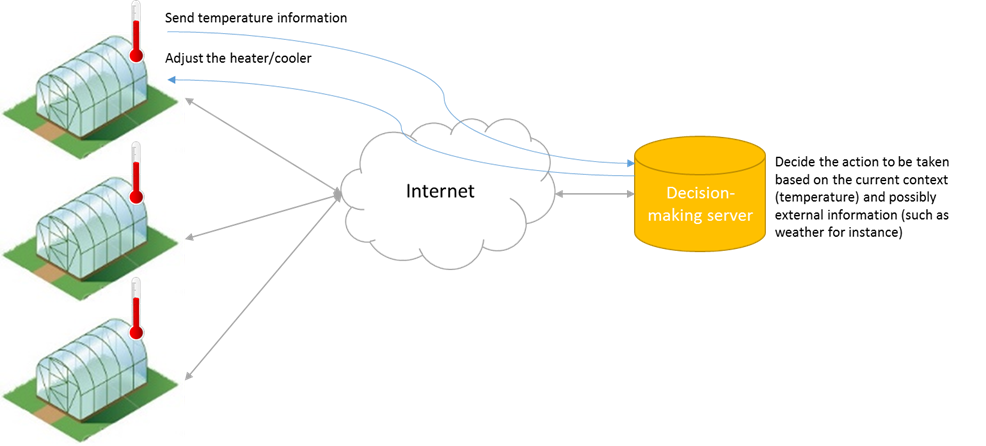
\includegraphics[width=0.9\columnwidth]{images/smart_farm.png}
\caption{Smart-farm scheme}
\label{figure:smartfarm}
\end{figure}
\end{center}


\section{Discussion}
\label{section:discussion}

better integration to provide true improvment upon golo
lots of improvement to make on the context management system so that it would be possible use it at its full potential
refining at the dynamic object or structure level and latter for classes if golo happens to support it in the future

\section{Conclusion \& Perspectives}
\label{section:conclusion}


%
% Bibliography
%
\goodbreak
\bibliographystyle{plain}
\bibliography{bmaingret_PFE_2014_Report}


\end{document}

